\chapter{Physical Verification and Signoff}
\label{chap:physical_verification}

After the completion of physical implementation, the UART layout was subjected to a comprehensive verification process to ensure that the generated design satisfies timing, power integrity, layout correctness, and manufacturability requirements. The verification stages were performed using the integrated tools available in the OpenLane2 flow, including OpenRCX, OpenSTA, Magic, Netgen, and the manufacturability checker.

%%%%%%%%%%%%%%%%%%%%%%%%%%%%%%%%%%%%%%%%%%%%%%%%%%%%%%%%%%%%%%%

\section{Verification Flow}

The verification stages performed after routing are illustrated in Figure~\ref{fig:verification_flow}.

\begin{figure}[!htbp]
    \centering
    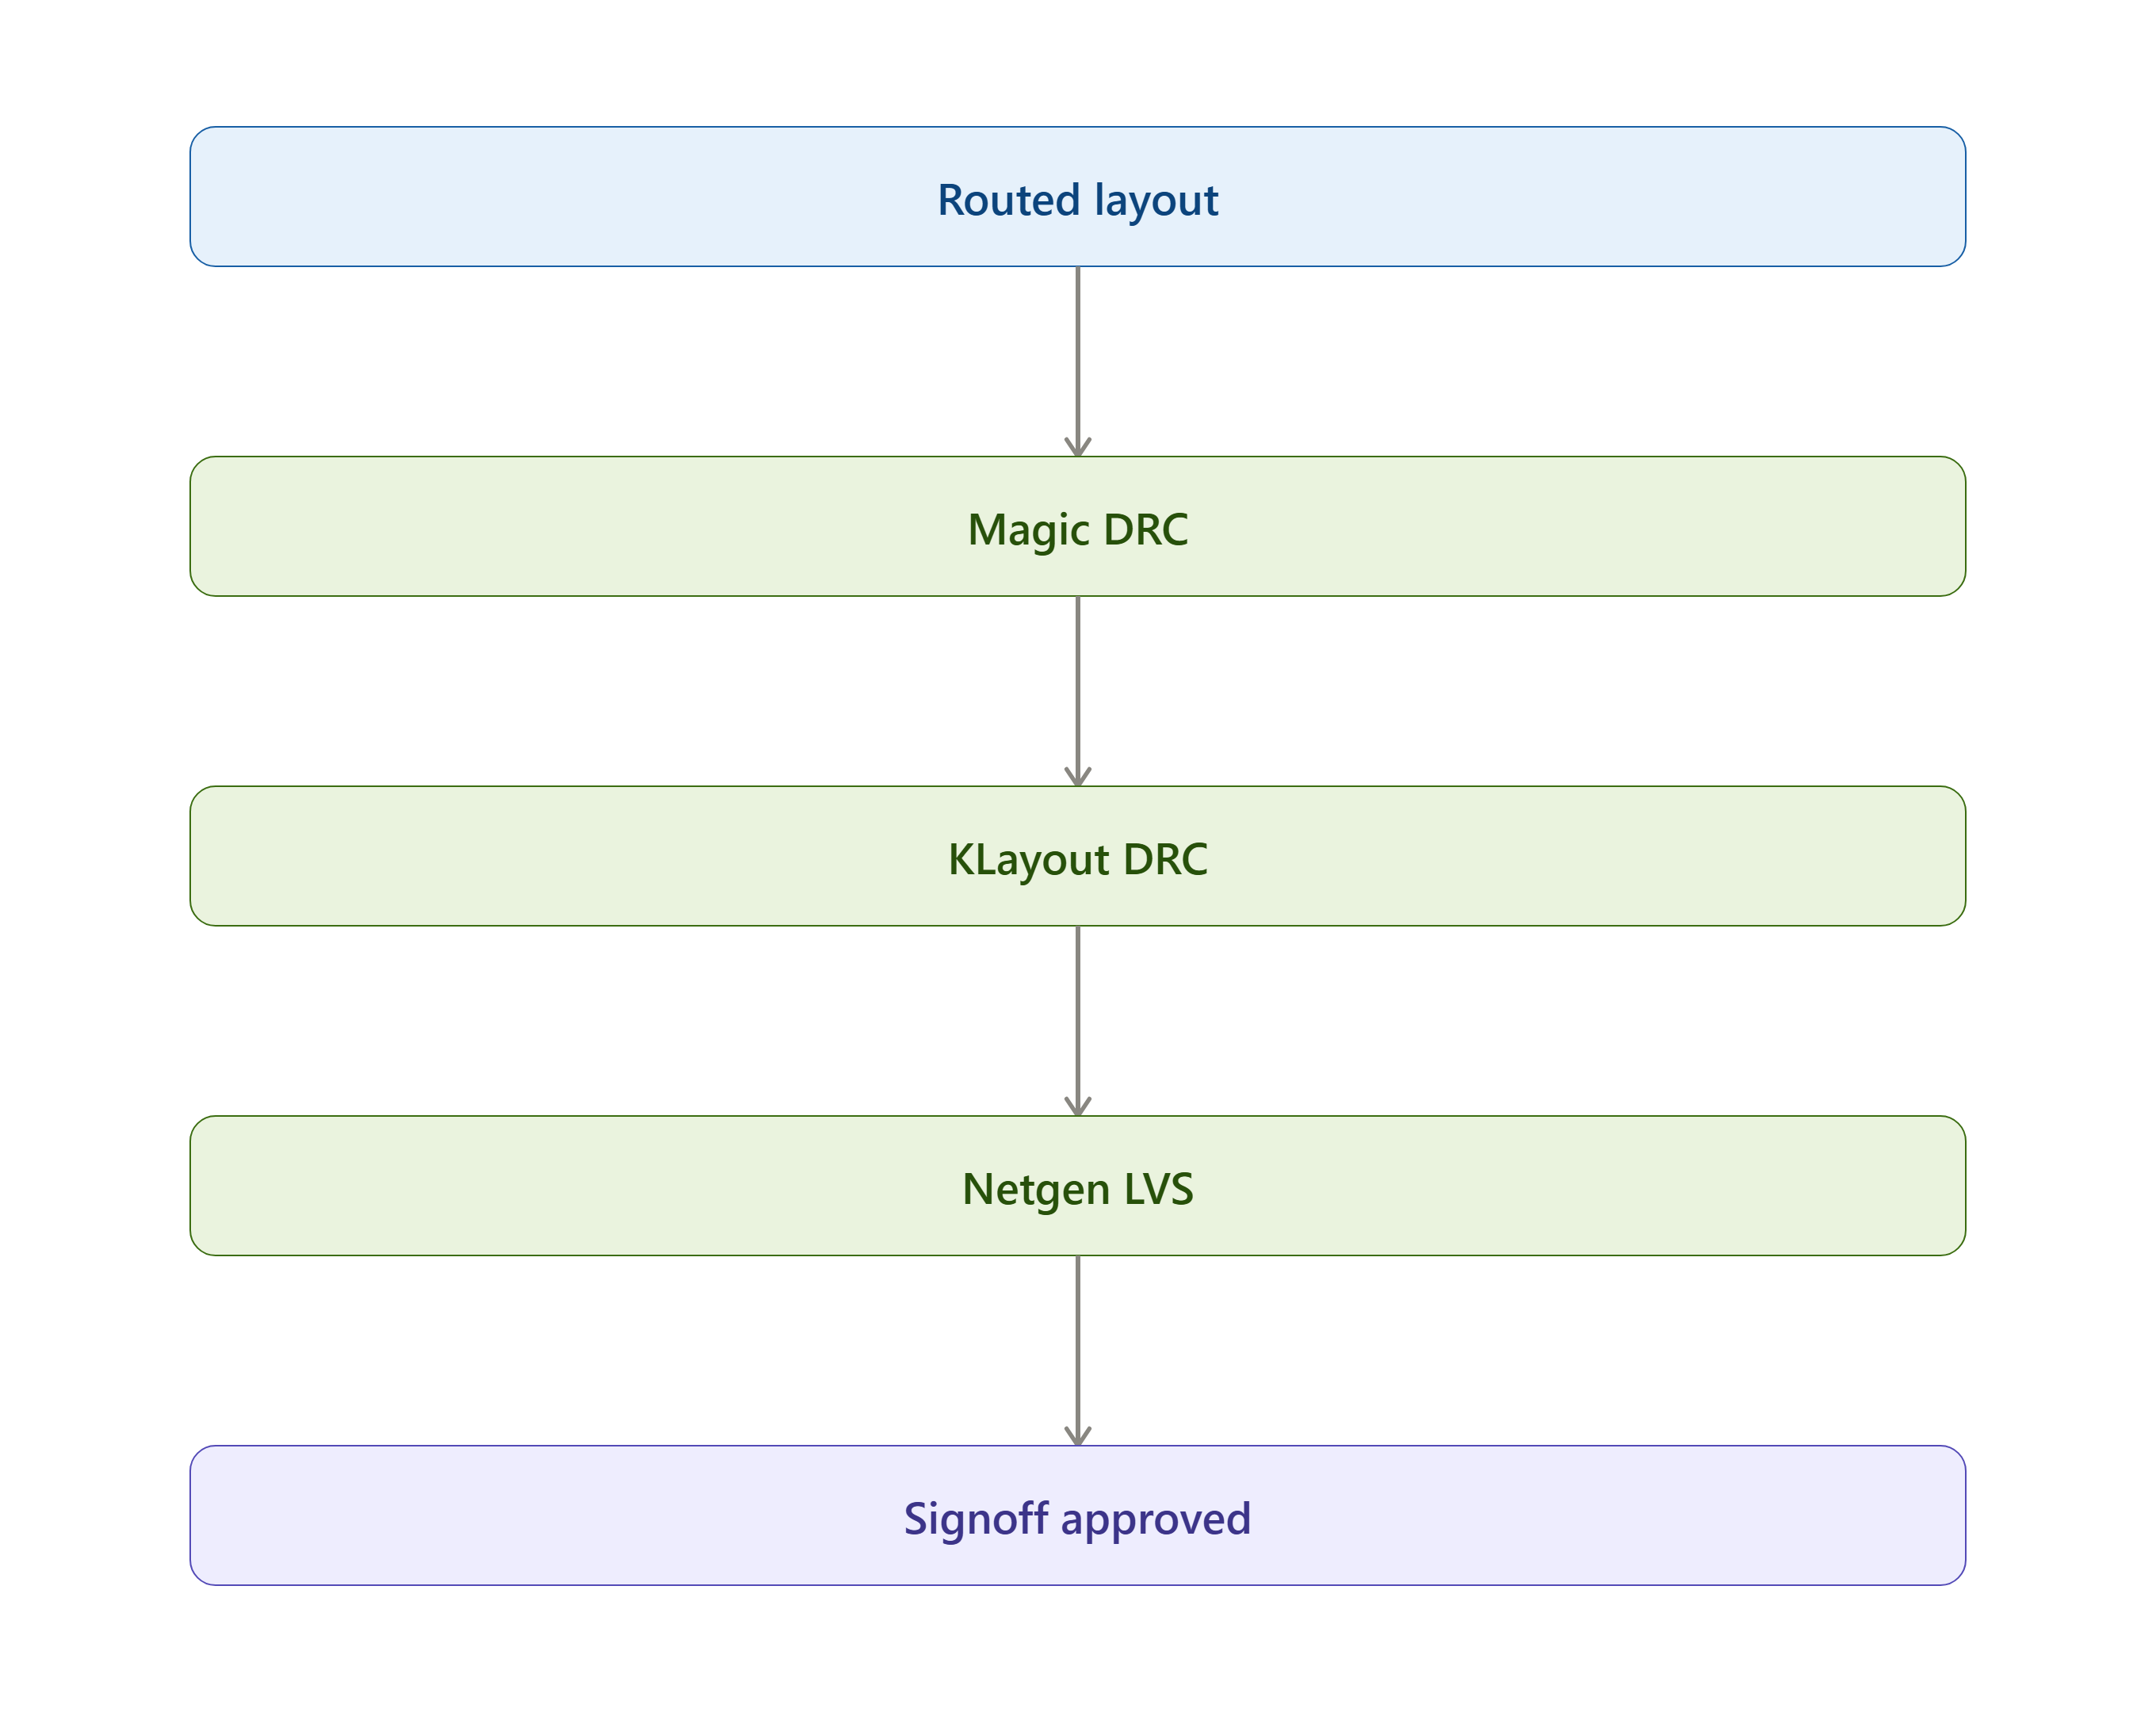
\includegraphics[width=0.86\textwidth]{images/physical_verification.png}
    \caption{Physical verification and signoff flow.}
    \label{fig:verification_flow}
\end{figure}

%%%%%%%%%%%%%%%%%%%%%%%%%%%%%%%%%%%%%%%%%%%%%%%%%%%%%%%%%%%%%%%

\section{RC Extraction}

After routing, parasitic resistance and capacitance associated with the interconnects were extracted using OpenRCX. The extracted parasitic information was stored in Standard Parasitic Exchange Format (SPEF) files and used for accurate post-layout timing analysis.

The RC extraction stage generated parasitic information for multiple process corners, as summarized in Table~\ref{tab:rcx_outputs}.

\begin{table}[!htbp]
\centering
\caption{Generated SPEF files}
\label{tab:rcx_outputs}
\begin{tabular}{ll}
\toprule
Operating Corner & Generated File\\
\midrule
Minimum & uart\_top.min.spef\\
Nominal & uart\_top.nom.spef\\
Maximum & uart\_top.max.spef\\
\bottomrule
\end{tabular}
\end{table}

The successful generation of all three SPEF files confirms that parasitic extraction was completed successfully without any extraction errors.

%%%%%%%%%%%%%%%%%%%%%%%%%%%%%%%%%%%%%%%%%%%%%%%%%%%%%%%%%%%%%%%

\section{Static Timing Analysis}

Static Timing Analysis (STA) was performed using the extracted parasitic information to verify timing performance under multiple operating corners.

The timing analysis evaluated setup and hold constraints across different process, voltage, and temperature (PVT) conditions. The analysis completed successfully without reporting critical timing violations, indicating successful timing closure after routing.

%%%%%%%%%%%%%%%%%%%%%%%%%%%%%%%%%%%%%%%%%%%%%%%%%%%%%%%%%%%%%%%

\section{IR Drop Analysis}

Power integrity analysis was performed to evaluate voltage drops across the power distribution network. The analysis confirmed that both the power (VPWR) and ground (VGND) networks maintain stable operating voltages throughout the design.

The measured voltage drops are summarized in Table~\ref{tab:irdrop_results}.

\begin{table}[!htbp]
\centering
\caption{IR-drop analysis results}
\label{tab:irdrop_results}
\begin{tabular}{lcc}
\toprule
Parameter & VPWR & VGND\\
\midrule
Worst Voltage & 1.79984 V & 0.000233 V\\
Average IR Drop & 0.0000416 V & 0.0000400 V\\
Worst IR Drop & 0.0001605 V & 0.0002330 V\\
Percentage Drop & 0.01\% & 0.01\%\\
\bottomrule
\end{tabular}
\end{table}

The observed voltage drop is extremely small, indicating a robust power distribution network suitable for reliable circuit operation.

%%%%%%%%%%%%%%%%%%%%%%%%%%%%%%%%%%%%%%%%%%%%%%%%%%%%%%%%%%%%%%%

\section{Design Rule Checking}

Magic was used to perform Design Rule Checking (DRC) on the routed layout. The generated layout was verified against the SKY130 manufacturing design rules.

The verification completed successfully with zero DRC violations.

\begin{table}[!htbp]
\centering
\caption{Magic DRC summary}
\label{tab:drc_summary}
\begin{tabular}{lc}
\toprule
Parameter & Result\\
\midrule
DRC Violations & 0\\
Verification Status & PASS\\
\bottomrule
\end{tabular}
\end{table}

%%%%%%%%%%%%%%%%%%%%%%%%%%%%%%%%%%%%%%%%%%%%%%%%%%%%%%%%%%%%%%%

\section{Layout Versus Schematic Verification}

Netgen was used to perform Layout Versus Schematic (LVS) verification. This step compares the extracted layout netlist against the synthesized gate-level netlist to ensure logical equivalence.


The LVS verification completed successfully, confirming that the physical layout matches the intended circuit implementation.

\begin{table}[!htbp]
\centering
\caption{LVS verification summary}
\label{tab:lvs_summary}
\begin{tabular}{lc}
\toprule
Parameter & Result\\
\midrule
Layout Matches Schematic & PASS\\
Verification Status & PASS\\
\bottomrule
\end{tabular}
\end{table}

%%%%%%%%%%%%%%%%%%%%%%%%%%%%%%%%%%%%%%%%%%%%%%%%%%%%%%%%%%%%%%%

\section{Final GDSII Layout}

The verified UART layout was exported in GDSII format after successful completion of all implementation and verification stages. Figure~\ref{fig:gds_layout} shows the final layout viewed in KLayout.

\begin{figure}[!htbp]
    \centering
    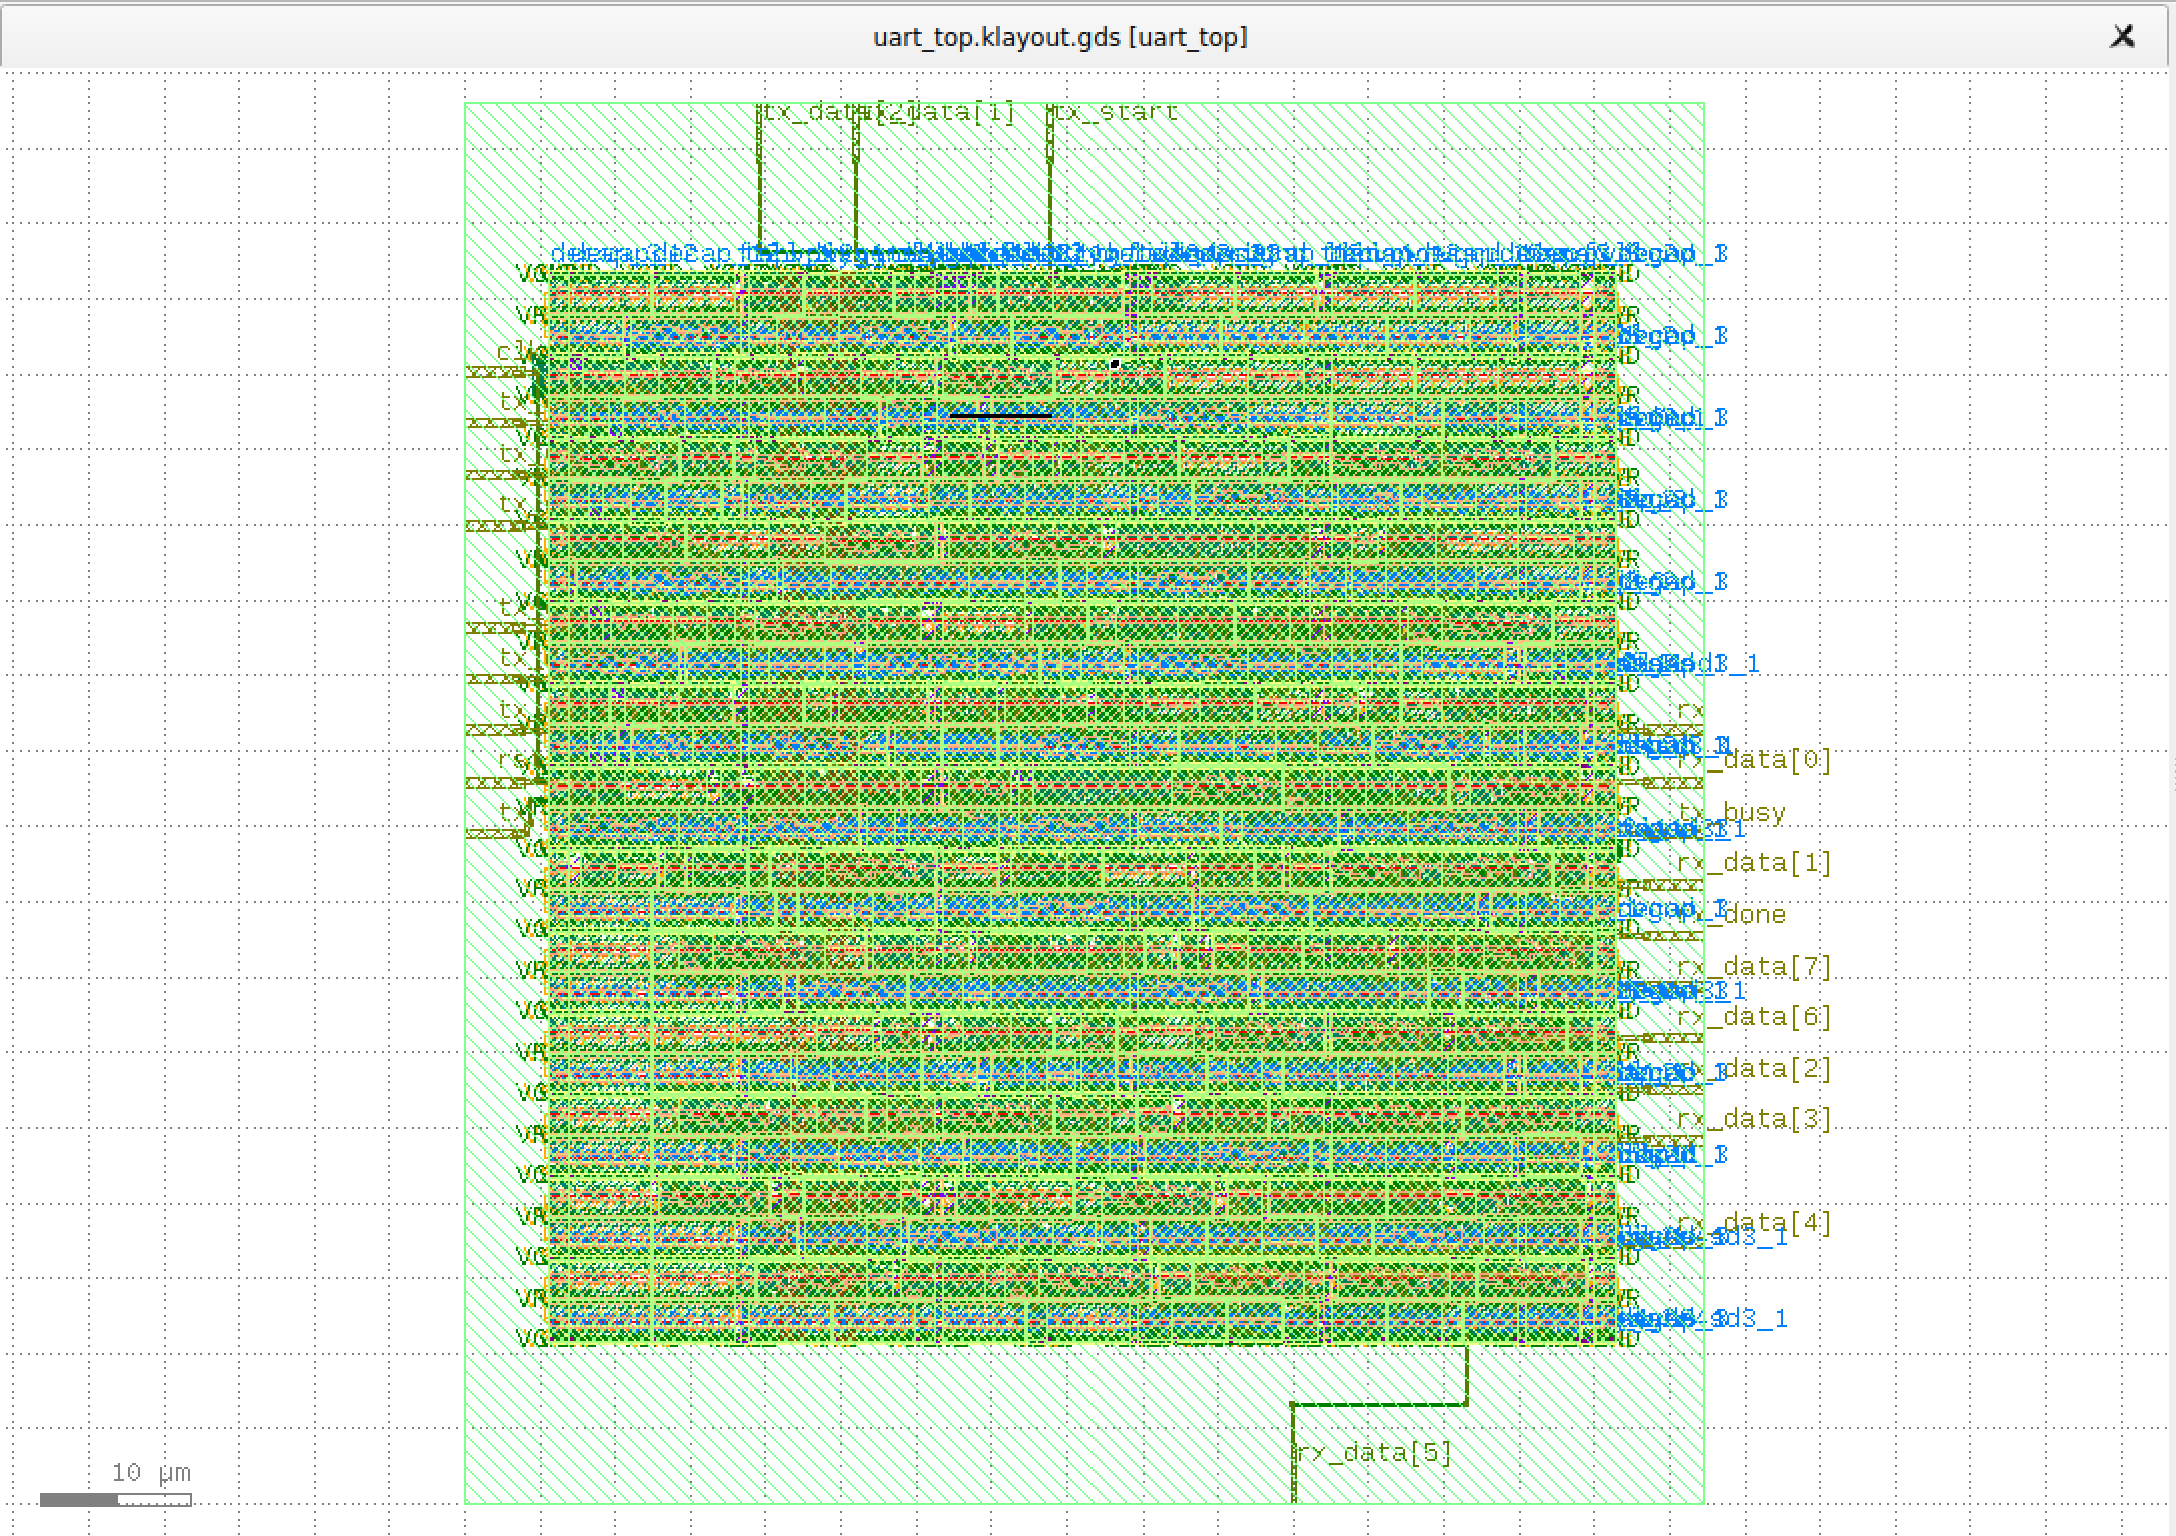
\includegraphics[width=0.92\textwidth]{images/Final_GDSII_Layout_in_KLayout.png}
    \caption{Final GDSII layout of the UART IP core viewed in KLayout.}
    \label{fig:gds_layout}
\end{figure}



\section{Manufacturability Assessment}

The final manufacturability report summarizes the overall fabrication readiness of the design by combining the results of antenna checking, DRC, and LVS verification.


The verification summary is presented in Table~\ref{tab:manufacturability}.

\begin{table}[!htbp]
\centering
\caption{Manufacturability verification summary}
\label{tab:manufacturability}
\begin{tabular}{lc}
\toprule
Verification Stage & Status\\
\midrule
Antenna Check & PASS\\
Magic DRC & PASS\\
Netgen LVS & PASS\\
Manufacturability & PASS\\
\bottomrule
\end{tabular}
\end{table}

The successful completion of all verification stages confirms that the UART ASIC implementation satisfies the required design rules and verification checks. The generated layout is therefore considered suitable for fabrication using the SKY130 process.